\subsection{GPUs}\label{subsec:gpus}

We briefly review NVIDIA GPUs%
\footnote{A more comprehensive introduction to GPUs themselves and CUDA programming is available in~\cite{10.5555/2935593}.}
in order that the performance criteria we measure in~\cref{sec:methodology} are intelligible.

A GPU consists of many simple processors, called streaming multiprocessors (SMs), which are comprised by many compute \textit{cores} that run at relatively low clock speeds%
\footnote{For example, individual NVIDIA GTX-1080 Ti cores run at $\sim$1500MHz.}.
Each compute core in an SM can execute one floating-point or integer operation per clock cycle.
See ~\cref{fig:fermi_arch} for a diagram of NVIDIA's Fermi architecture, where each SM consists of 32 cores, 16 load/store (LD/ST) units, four special-function units (SFUs) which compute transcendental functions (such as $\sin$, $\cos$, $\exp$), a relatively large register file%
\footnote{For example, Intel's Haswell architecture supports 168 integer and 168 floating-point registers.}%
, and thread control logic (to be discussed in the proceeding).
Each SM has access to local memory, several cache levels, and global memory.
In the Fermi architecture (and subsequent architectures) this local memory is configurable in software;
a fraction of it can be apportioned as either local memory or L1 cache (for workloads that query global memory in excess of local memory).
One final feature worth mentioning, though irrelevant for us here, is the L2 cache's atomic \code{read-modify-write} facilities;
this enables sharing data across groups of threads more efficiently than possible in conventional CPUs%
\footnote{On a CPU, atomic \code{test-and-set} instructions manage a semaphore, which itself manages access to memory (therefore incurring a cost of at least two clock cycles).}.

Such an architecture, particularly suited to maximizing throughput, necessitates a programming model distinct from that of a conventional, general purpose processor architecture.
A unit of computation deployed to a GPU is called a \textit{kernel}; kernels can be defined using NVIDIA's Compute Unified Device Architecture (CUDA) extensions to C, C++, and FORTRAN%
\footnote{In fact CUDA compiles down to a virtual machine assembly code (by way of \code{nvcc}) for a virtual machine called the Parallel Thread Execution (PTX) virtual machine. So, in effect, it's compilers all the way down.}.
Compiled kernels are comprised by many \textit{threads} that start with the same instruction(s) in parallel;
NVIDIA describes this addition to Flynn's taxonomy~\cite{5009071} as Single Instruction Multiple Thread (SIMT)%
\footnote{They key difference between SIMD and SIMT is that while in SIMD all vector elements in a vector instruction execute synchronously, threads in SIMT can diverge; branches are handled by predicated instructions~\cite{cuda_toolkit}.}.
The large register file enables very fast thread context switching ($\sim$25 microseconds on the Fermi architecture~\cite{Glaskowsky2009NVIDIAS}), performed by a centralized hardware thread scheduler.
Multiple threads are grouped into blocks (SMs are single tenant with respect to blocks) and blocks are grouped into \textit{grids} (grids execute a single kernel).
All threads in a block, by virtue of running on the same SM, coordinate (execute in arbitrary order, concurrently, or sequentially) and share memory.
Thread blocks are partitioned into \textit{warps} of 32 threads;
it is these warps that are dispatched by the warp scheduler (see~\cref{fig:cuda_cores}) and starting with the Fermi architecture two warps can be executed concurrently on the same SM in order to increase utilization%
\footnote{I.e. one warp can occupy the compute cores while the other occupies the SFUs or Load/Store units.}.

\begin{figure}
    \centering
    \begin{subfigure}{\linewidth}
        \centering
        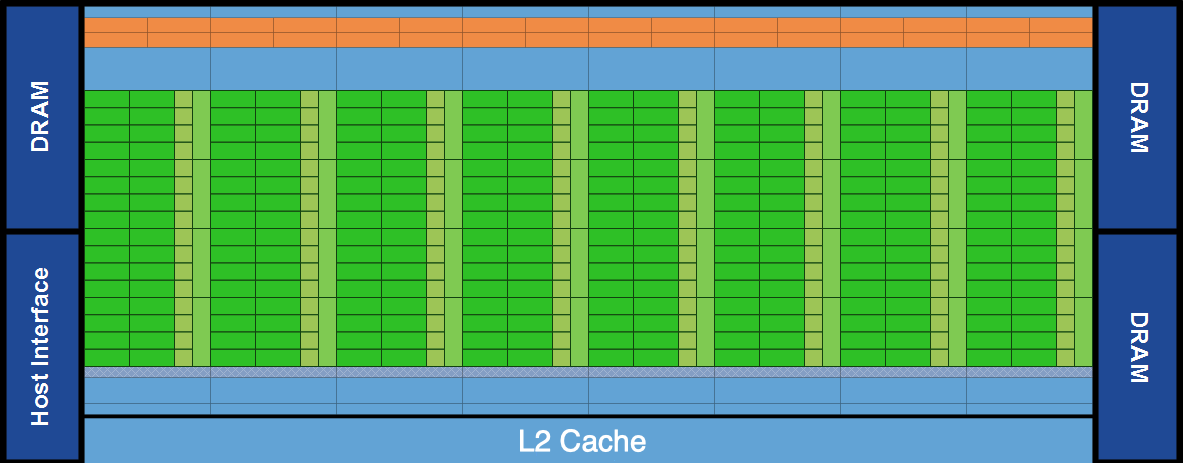
\includegraphics[width=\linewidth]{figures/fermi_arch.png}
        \caption{Eight (of 16) SM in the Fermi architecture (remaining 8 are symmetrically placed around the L2 cache)}
        \label{fig:top_half_ferm_arch}
    \end{subfigure}
    \\[3ex]
    \begin{subfigure}{\linewidth}
        \centering
        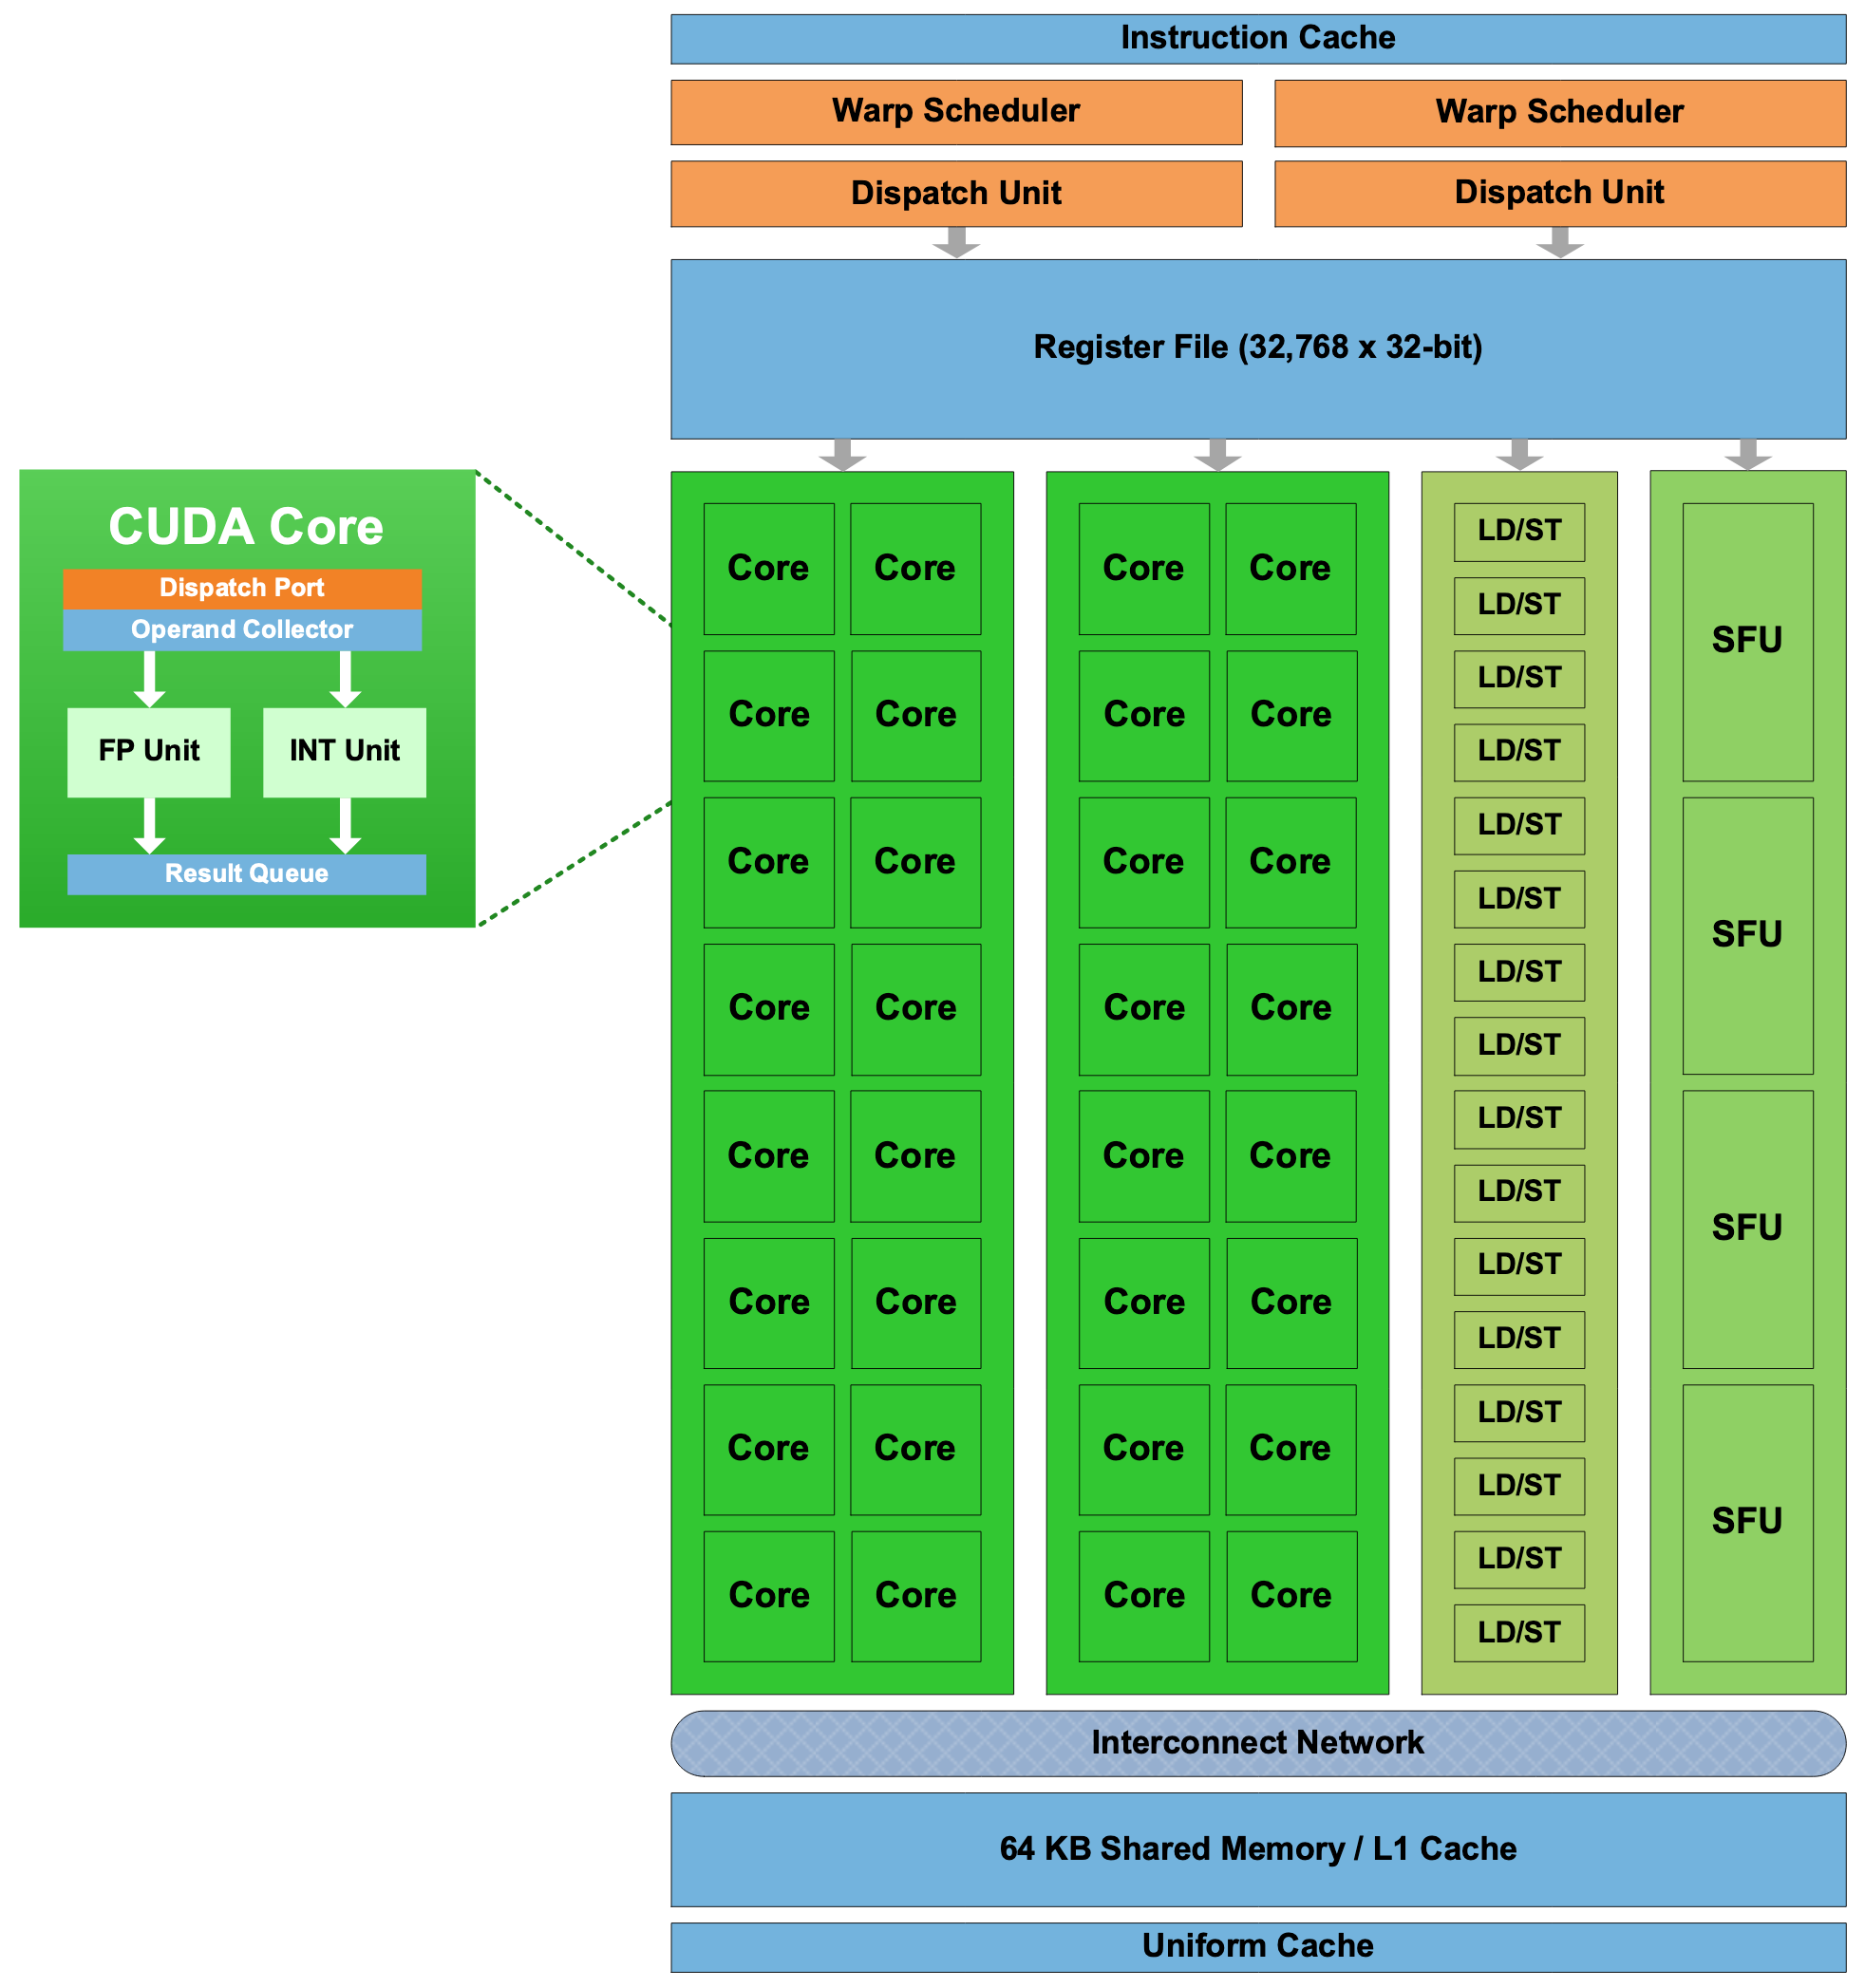
\includegraphics[width=\linewidth]{figures/cuda_cores.png}
        \caption{An individual Fermi SM}
        \label{fig:cuda_cores}
    \end{subfigure}
    \caption{NVIDIA Fermi Architecture~\cite{5751939}}
    \label{fig:fermi_arch}
\end{figure}


We present an example CUDA program in~\cref{fig:cuda_hello_world} to illustrate some of the artifacts of the CUDA threading model.
The premise of the program is performing an element-wise sum of two $32 \times 48$ entry matrices.
Note that all of the data weighs in at  $3 \times 32 \times 48 \times 4 = 18$ kilobytes (well within the bounds of shared memory of any one SM).
The actual work of the summing is partitioned across a grid of 6 thread blocks, each containing $16 \times 16$ threads.
Such a partitioning means each thread can be logically responsible for exactly one sum and therefore the kernel is quite simple (see~\cref{lst:cuda_hello_world}).
Within the context of a kernel, each thread is uniquely identified by it's multi-index in the thread hierarchy (\code{threadIdx} and \code{blockIdx}).
Hence, to carry out the sum, the kernel maps this multi-index to the physical address of the data%
\footnote{In CUDA C/C++ data is laid out in row-major order but this is not fixed (in CUDA FORTRAN the data is laid out in column-major order).}.
This (grid, block, thread)$\rightarrow$data mapping is, in effect, the mechanism that implements the SIMT architecture.
Note that, since each block is allocated to exactly one SM, this sum will take $\left( 16 \times 16 \right) \div 16 = 16$ clock cycles on the Fermi architecture;
better throughput could be achieved by increasing the number of blocks (and therefore the number of SMs assigned work).

\begin{figure}
    \centering
    \begin{subfigure}{\linewidth}
        \centering
        \cfile{code/hello_world_kernel.c}
        \caption{CUDA code to be compiled by \mintinline{c}{nvcc}.
        Note differences \mintinline{c}{__global__} and \mintinline{c}{matrix_sum<<,>>} from standard C.
        }
        \label{lst:cuda_hello_world}
    \end{subfigure}
    \\[3ex]
    \begin{subfigure}{\linewidth}
        \centering
        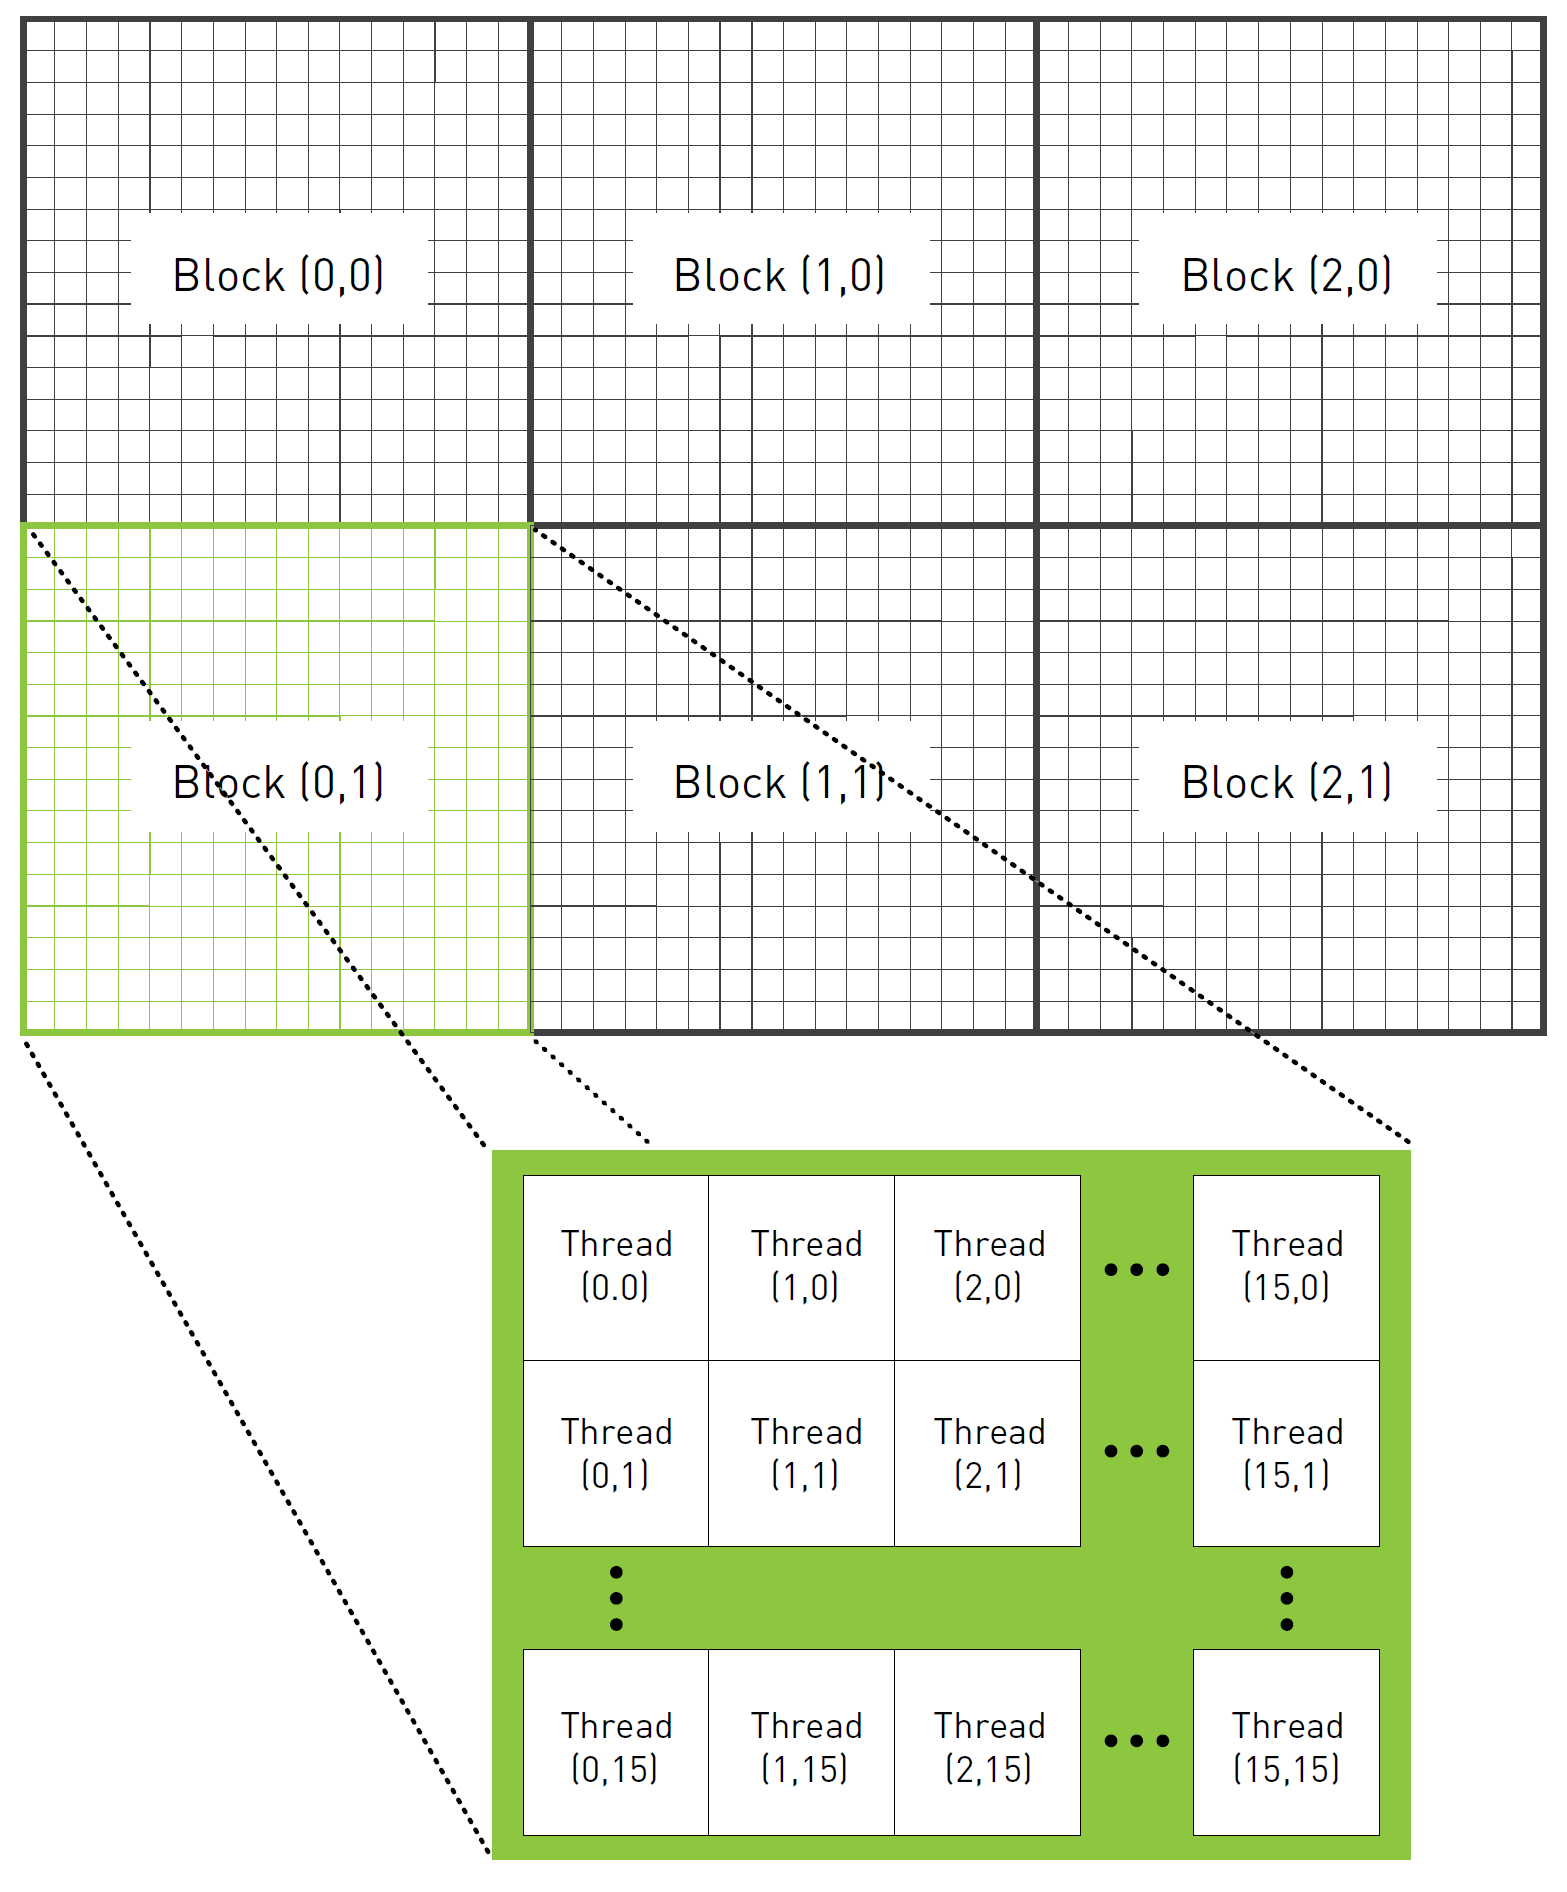
\includegraphics[width=\linewidth]{figures/matrix_thread.png}
        \caption{Mapping from thread and block to matrix element~\cite{10.5555/1891996}.}
        \label{fig:matrix_thread}
    \end{subfigure}
    \caption{Canonical CUDA "hello world" kernel (matrix addition).}
    \label{fig:cuda_hello_world}
\end{figure}


\subsection{Graph compilers}\label{subsec:graph-compilers}

DL frameworks primarily function as graph compilers;
they compile abstract dataflow and compute graphs into sequences of operations that execute on various hardware architectures.
They typically also implement some ``quality of life'' abstractions like \code{Tensor}%
\footnote{A tensor in this context is a data structure similar to a multidimensional array that supports some useful operations (e.g. slicing, flattening, index permutation). Most DL frameworks also abstract memory layout on hardware behind this abstraction.} and include utilities useful for the training of DL models (e.g. optimizers and data loaders).
Here we focus in particular on the graph compiler functionality.

DL graph compilers are distinct from other dataflow compilers (such as VHDL and Verilog\footnote{Verilog and Very High Speed Integrated Circuit Hardware Description Language (VHSIC-HDL or VHDL) are specification languages for specifying circuits on field programmable gate arrays.}); in addition to keeping account of how the data streams through the compute graph, they also keep account of how the gradients of the data stream through the graph (i.e.\ the \textit{gradient-flow}).
This is called \textit{automatic differentiation} (often shortened to \textit{autodiff}).
In principle autodiff is implemented by using the rules of Newton's calculus to calculate the derivatives of primitive functions and the chain rule to calculate derivatives of compositions of primitive functions.
There are two types of autodiff: \textit{forward mode} (or \textit{forward accumulation}) and \textit{reverse mode} (or \textit{reverse accumulation})%
\footnote{Briefly, for a composition of functions $y=f(g(h(x)))$, forward mode evaluates the derivative $y'(x)$, as given by the chain rule, inside-out while reverse mode evaluates the derivative outside-in. For those familiar with functional programming, these operations correspond to \code{foldl} and \code{foldr} on the sequence of functions with $\partial_x$ as the operator.}.
Reverse mode autodiff enables the framework to effectively calculate the gradients of parameters of a neural network with respect to some relevant loss or objective function.
Note that such gradients can be \textit{back-propagated} through the neural network in order to adjust the parameters of the neural network such that it minimizes the loss\footnote{In which case, it is in fact the negatives of the gradients that are back-propagated.} or maximizes the objective.

Dataflow graphs (and their corresponding gradient-flow graphs) can be specified either statically, with fan-in and fan-out for all functions predetermined, or dynamically, where connections between functions are determined ``on-the-run''.
There are advantages and disadvantages to both specification strategies.
Static specifications tightly constrain\footnote{For example, branches and loops are cumbersome to specify statically.} the intricacy of the dataflow graph but, obversely, can be leveraged to improve performance and scalability~\cite{le2019tflms,Pradelle2017PolyhedralOO}.
TensorFlow (prior to v2.0) is an example of a DL framework that compiles statically specified graphs.
Conversely, dynamic specifications can be very expressive and user friendly, including such conveniences as runtime debugging, but are much more difficult to optimize.
PyTorch is an example of a DL framework that supports dynamic specification.
Both PyTorch and TensorFlow also support just-in-time (JIT) compilation strategies (TorchScript and XLA respectively);
such JIT compilers strike a balance between fluency and scalability.
In this work we investigate TorchScript (see~\cref{sec:methodology}).

It warrants mentioning that, in addition to vertically integrated DL frameworks (i.e.\ specification language and hardware compiler), recently there has been work on intermediate byte code representations for dataflow graphs that arbitrary compiler ``frontends'' can target.
The Multi-Level Intermediate Representation (MLIR)~\cite{lattner2020mlir} project has goals that include supporting dataflow graphs, optimization passes on those graphs and hardware specific optimizations%
\footnote{Interestingly enough, the project is headed by Chris Lattner who, in developing LLVM, pioneered the same ideas in general purpose programming languages.}.
Stripe~\cite{zerrell2019stripe} is a polyhedral compiler%
\footnote{A polyhedral compiler models complex programs (usually deeply nested loops) as polyhedra and then performs transformations on those polyhedra in order to produce equivalent but optimized programs~\cite{Griebl98codegeneration}.}
that aims to support general machine learning kernels, which are distinguished by their high parallelism with limited mutual dependence between iterations.
Tensor Comprehensions~\cite{vasilache2018tensor} is an intermediate specification language (rather than intermediate byte code representation) and corresponding polyhedral compiler;
the syntax bears close resemblance to Einstein summation notation and the compiler supports operator fusion and specialization for particular data shapes.
Finally, Tensor Virtual Machine (TVM)~\cite{10.5555/3291168.3291211} is an optimizing graph compiler that automates optimization using a learning-based cost modeling method that enables it to efficiently explore the space of low-level code optimizations.